Structured Query Language (SQL) is generally considered the most effective
programming language for managing structured data. In our system, there are
five fundamental entities:

\begin{enumerate}
  \item Tool - represents the underlying tool utilised during the decomposition
    process. It encompasses the specific software or framework for breaking
    down a system into smaller components.
  \item Language - signifies the programming languages that can be targeted for
    decomposition. It encapsulates the various programming languages that the
    system supports for component extraction.
  \item Result - denotes whether a decomposition job succeeded or encountered
    any issues.
  \item Decomposition - encapsulates the actual decomposition and includes all
    the necessary data to represent it comprehensively.
  \item Service - represents each microservice within the system.
\end{enumerate}

The relationships between these entities are illustrated in
\Cref{fig:database-model}, visually depicting their interconnections.

\begin{figure*}[!htb]
  \caption{Database Model}
  \label{fig:database-model}
  \centering
  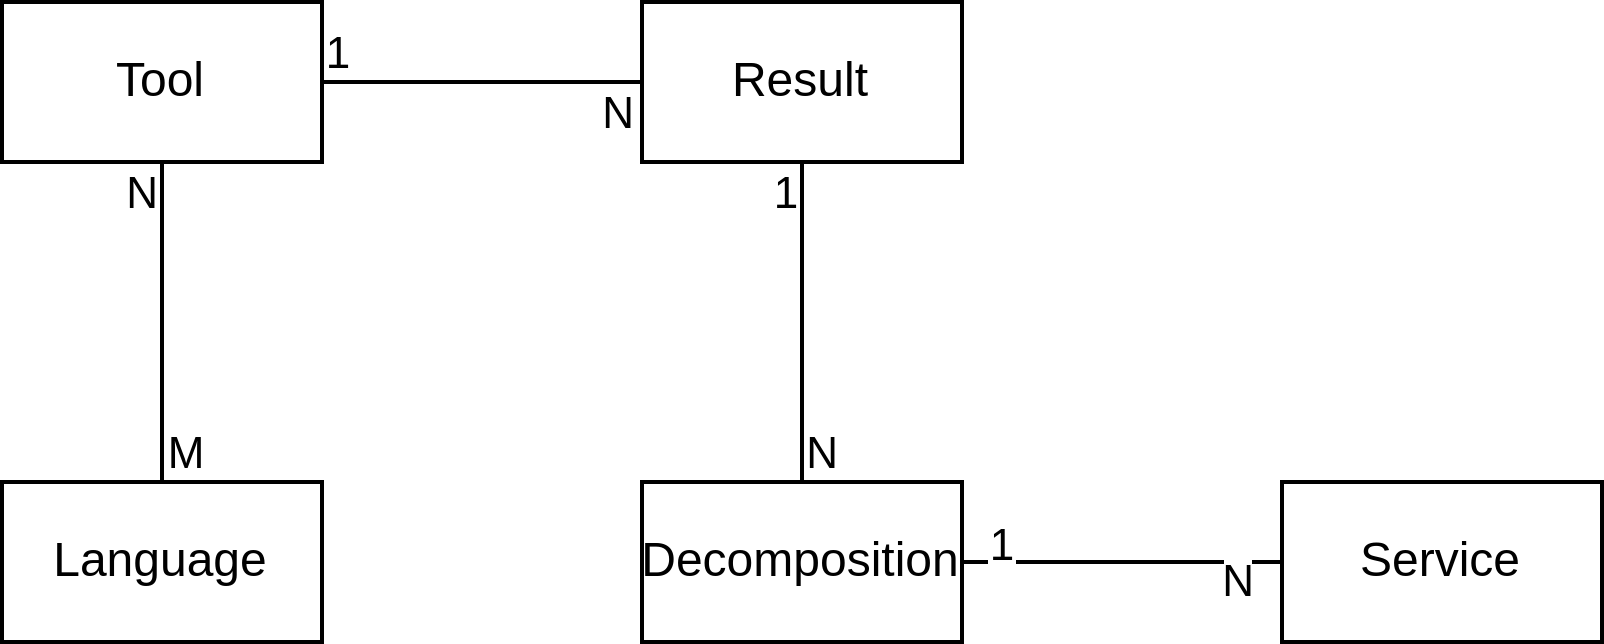
\includegraphics[width=\textwidth]{thesis-er.drawio}
\end{figure*}
